\subsubsection{UC8 - Disconnessione dal servizio}
\begin{figure}[h]
	\centering
	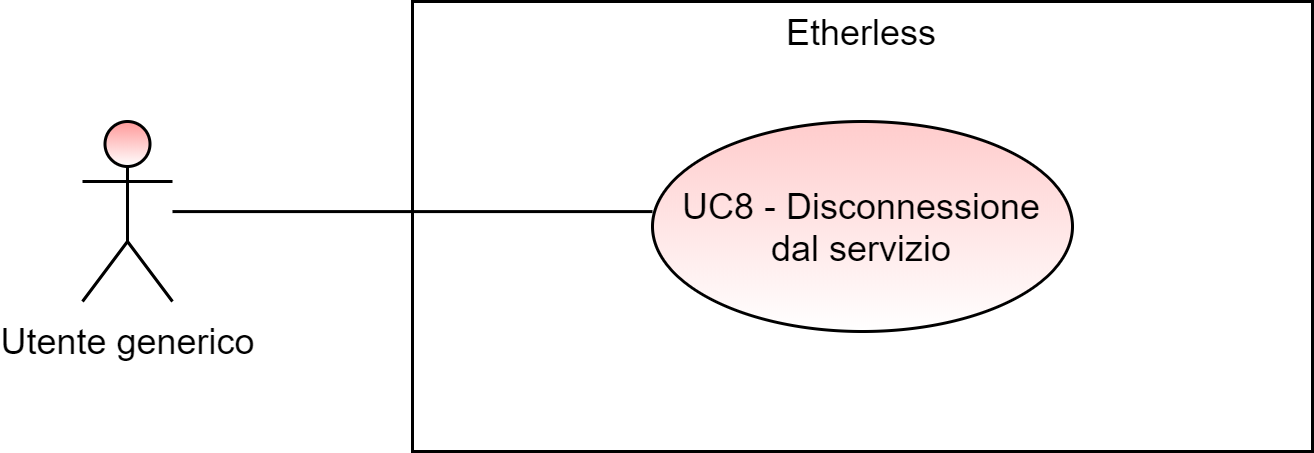
\includegraphics[scale=\ucs]{./res/img/UC8G.png}
	\caption {UC8 - Disconnessione dal servizio: schema generale}
\end{figure}
\begin{itemize}
	\item \textbf{Attori primari:} \ua{};
	\item \textbf{Descrizione:} l’utente richiede la disconnessione dal servizio eseguendo il comando \logout{}. Il sistema effettua la disconnessione; 
	\item \textbf{Scenario principale:} 
	\begin{itemize}
		\item l'utente inserisce correttamente ed esegue il comando \logout{}; 
		\item l'utente viene disconnesso dal servizio. 
	\end{itemize}
	\item \textbf{Precondizione:} l’utente è stato autenticato correttamente e richiede di essere disconnesso; 
	\item \textbf{Postcondizione:} l’utente viene disconnesso con successo..
\end{itemize}